
\begin{question}[name=Oppgave, topic=dioder]
	Tegn symbolene for følgende komponenter.
	\begin{enumerate}[label=\roman*)]
		\item Halvlederdiode
		\item LED
		\item Zenerdiode
	\end{enumerate}
\end{question}

\vspace{0.5cm} % Add space after the solution

\begin{solution}[name=Løsningsforslag oppgave]
Symboler vist i Figur \ref{fig:diodeSymb}.
	\begin{figure}[H]
		\centering
		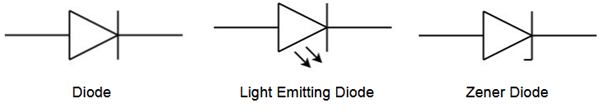
\includegraphics[width=0.7\textwidth]{diode/figurer/oppgave1.png}
		\caption{Eksempel på forskjellige symboler for dioder.}
		\label{fig:diodeSymb}
	\end{figure}
\end{solution}

\vspace{0.5cm} % Add space after the solution

\begin{question}[name=Oppgave, topic=dioder]
Hva betyr de følgende begrepene i sammenheng med dioder? Svar på spørsmålet og tegn eksempel.
	\begin{enumerate}[label=\roman*)]
		\item Lederetning
		\item Sperreretning
		\item Anode
		\item Katode
		\item Zenerspenning
	\end{enumerate}
\end{question}

\vspace{0.5cm} % Add space after the solution

\begin{solution}[name=Løsningsforslag oppgave]
	\begin{enumerate}[label=\roman*)]
		\item Diode koblet slik at den leder strøm
			\begin{figure}[H]
			\centering
			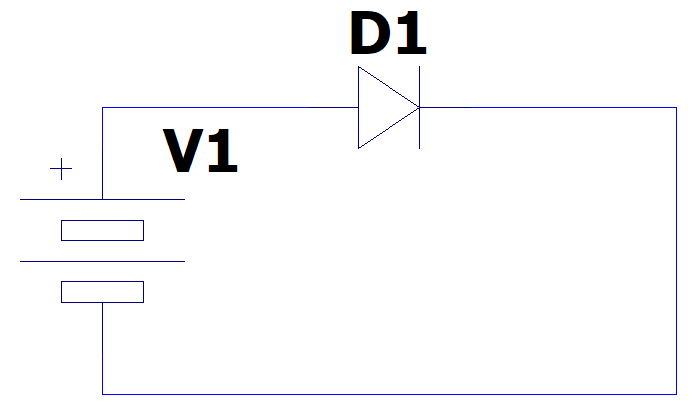
\includegraphics[width=0.4\textwidth]{diode/figurer/lederetning.png}
			\caption{Diode koblet i lederetning}
			\label{fig:lede}
		\end{figure}
		\item Diode koblet slik at den ikke leder strøm
			\begin{figure}[H]
				\centering
				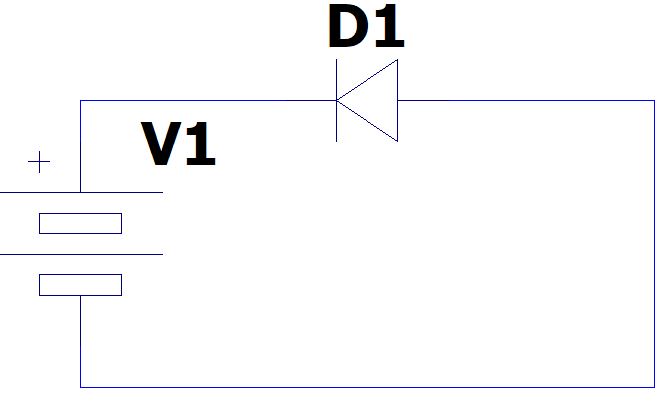
\includegraphics[width=0.4\textwidth]{diode/figurer/sperreretning.png}
				\caption{Diode koblet i sperreretning}
				\label{fig:sperre}
			\end{figure}
		\item Anode er siden så hvis man kobler den til den positive siden av en kilde, så vil dioden lede. Strømmen går fra anode til katode
		
			\begin{figure}[H]
				\centering
				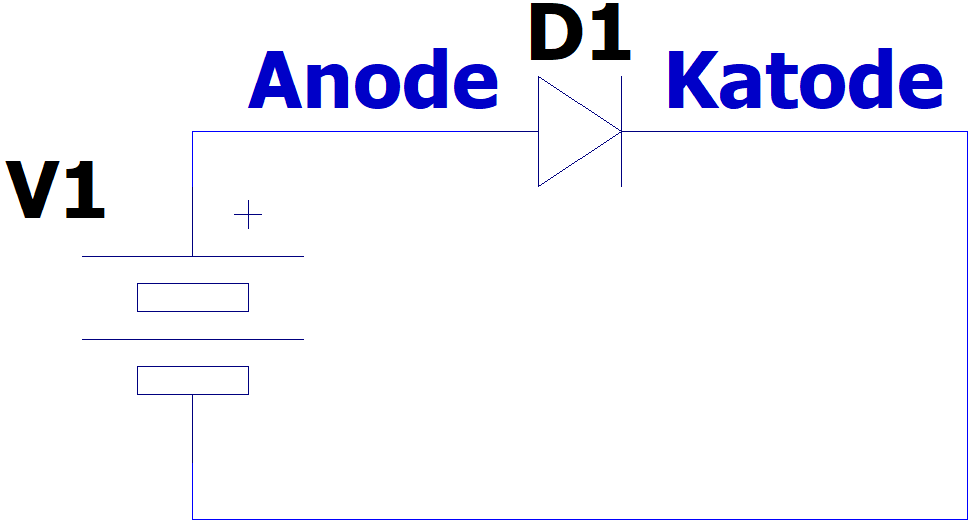
\includegraphics[width=0.4\textwidth]{diode/figurer/anodekatode.png}
				\caption{Anode og katode på diode}
				\label{fig:anoKato}
			\end{figure}
		\item Dersom dioden leder er katoden koblet til den negative siden av kilden som vist i Figur \ref{fig:anoKato}
		\item Zenerspenning er spenningen hvor en zenerdiode begynner å lede strøm i sperreretning, og kan stabiliserer spenningen i kretsen.
	\end{enumerate}
\end{solution}

\vspace{0.5cm} % Add space after the solution

\begin{question}[name=Oppgave, topic=dioder]
	Beskriv tre bruksområder for en halvlederdiode.
\end{question}

\vspace{0.5cm} % Add space after the solution

\begin{solution}[name=Løsningsforslag oppgave]
	\begin{enumerate}[label=\roman*)]
		\item Sperre for strøm i én retning
		\item For å beskytte transistorer og andre følsomme komponenter, kobles dioden som en friløpsdiode når den brukes sammen med en induktiv last.
		\item Likerette AC til DC
	\end{enumerate}
\end{solution}

\vspace{0.5cm} % Add space after the solution

\begin{question}[name=Oppgave, topic=dioder]
	En LED har et spenningsfall i lederetning på $2,5 [V]$ og det kreves en strøm på $15 [mA]$ for at den skal lyse. Den tilkoblede spenningskilden har en spenning ut på $15 [V]$.
	
	Beregn størrelsen på seriemotstanden til dioden.
\end{question}

\vspace{0.5cm} % Add space after the solution

\begin{solution}[name=Løsningsforslag oppgave]
Først finner vi spenningsfallet vi må ha over motstanden for at dioden skal ha et spenningsfall på $2,5 [V]$.


\[U_{R-serie}=U_{Kilde}-U_{LED}=15-2,5=12,5 [V]\]

Strømmen resistansen skal sørge for å begrense strømmen i kretsen til $15 [mA]$. Finner størrelsen på resistansen

\[R_{Serie}=\frac{U_{R-serie}}{I_{LED}}=\frac{12,5}{15\cdot10^{-3}}=830 [\Omega]\]

\end{solution}

\vspace{0.5cm} % Add space after the solution

\begin{question}[name=Oppgave, topic=dioder]
En likeretterdiode har et spenningsfall på $0,7 [V]$ over seg i lederetning. Hvor stor effekt omsettes det i dioden når strømmen er $2 [A]$?
\end{question}

\vspace{0.5cm} % Add space after the solution


\begin{solution}[name=Løsningsforslag oppgave]
\[P=U\cdot I = 0,7\cdot2=1,4 [W]\]
	
\end{solution}

\vspace{0.5cm} % Add space after the solution

\begin{question}[name=Oppgave, topic=dioder]
	Hvilken av kretsene vist i Figur \ref{fig:3kretser} er koblet slik at dioden står i lederetning?
	
	\begin{figure}[H]
		\centering
		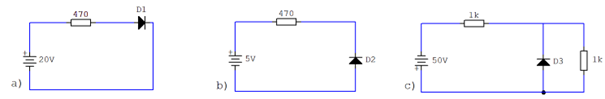
\includegraphics[width=0.9\textwidth]{diode/figurer/3Kretser.png}
		\caption{Tre forskjellige diodekretser}
		\label{fig:3kretser}
	\end{figure}
	
\end{question}

\vspace{0.5cm} % Add space after the solution

\begin{solution}[name=Løsningsforslag oppgave]
	Krets a) og c)
\end{solution}
\vspace{0.5cm} % Add space after the solution

\begin{question}[name=Oppgave, topic=dioder]
Hvilken spenning vil man måle mellom punkt1 og punkt2 i Figur \ref{fig:10Dserie}.

	\begin{figure}[H]
		\centering
		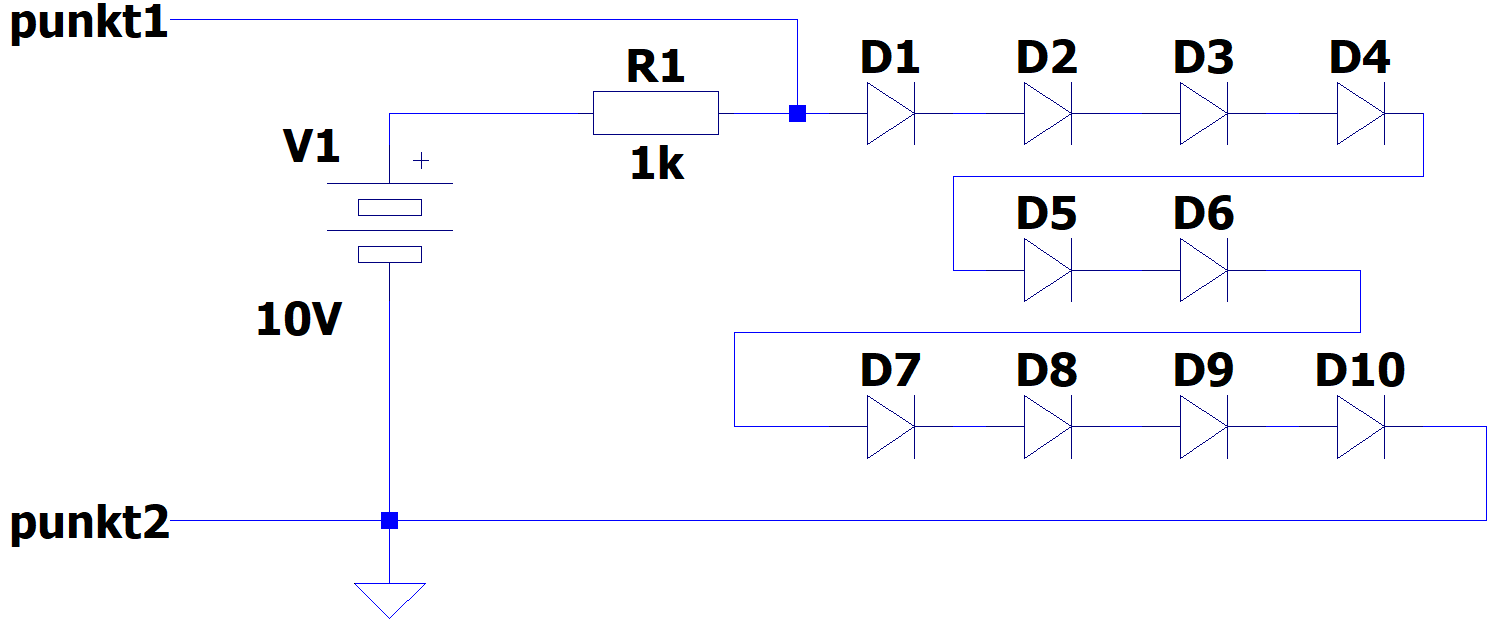
\includegraphics[width=0.7\textwidth]{diode/figurer/10SerieD.png}
		\caption{Krets med 10 dioder i serie}
		\label{fig:10Dserie}
	\end{figure}

\end{question}

\vspace{0.5cm} % Add space after the solution

\begin{solution}[name=Løsningsforslag oppgave]
	Summerer opp alle spenningsfallene i kretsen.
	\begin{multline*}
	U_{D_{tot}}=\sum_{i=1}^{10} U_{D_i}=\sum_{i=1}^{10}\cdot0,7 \Rightarrow \\	U_{D1}+U_{D2}+U_{D3}+U_{D4}+U_{D5}+U_{D6}+U_{D7}+U_{D8}+U_{D9}+U_{D10} \Rightarrow \\ U_{D_{tot}}=10\cdot0,7=7 [V]
		%SPICEmodell - DC-R10D.asc
	\end{multline*}
\end{solution}

\vspace{0.5cm} % Add space after the solution


\begin{question}[name=Oppgave, topic=dioder]
Hvilken spenning vil man måle mellom punkt1 og punkt2 i Figur \ref{fig:DserieParaMix}
	
	\begin{figure}[H]
	\centering
	\includegraphics[width=0.7\textwidth]{diode/figurer/6serieOgParaD.png}
	\caption{Krets med dioder i serie og parallell}
	\label{fig:DserieParaMix}
	\end{figure}
	
	
\end{question}

\vspace{0.5cm} % Add space after the solution

\begin{solution}[name=Løsningsforslag oppgave]
Siden spenningsfallet over grenenen $D1 \rightarrow D4$ er lik grenen $D5 \rightarrow D8$ kan man summere spenningsfallet over en av de for å finne spenningsfallet frem til anoden av $D9$.
\[U_{D1-D4}=U_{D1}+U_{D2}+U_{D3}+U_{D4}= 4\cdot0,7=2,8[V]\]

Benytter det beregnede spenningsfallet og legger til spenningsfallet over $U_{D9}$ og $U_{D10}$.

\[U_{D_{tot}}=U_{D1-D4}+U_{D9}+U_{D10}=2,8+0,7+0,7=4,2 [V]\]
%SPICEmodell - DC-R8D2S.asc

\end{solution}

\vspace{0.5cm} % Add space after the solution



\begin{question}[name=Oppgave, topic=dioder]
	Hvilke lamper lyser i Figur \ref{fig:hvilkenLampe}?
	
	\begin{figure}[H]
		\centering
		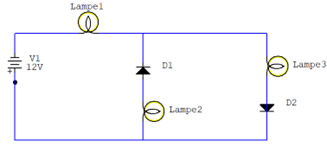
\includegraphics[width=0.7\textwidth]{diode/figurer/hvalyser.png}
		\caption{Lampekrets}
		\label{fig:hvilkenLampe}
	\end{figure}
	
	
\end{question}

\vspace{0.5cm} % Add space after the solution

\begin{solution}[name=Løsningsforslag oppgave]
Med utgangspunkt i spenningskildens polariet så vil lampe 1 og lampe 2 lyse.
	
\end{solution}

\vspace{0.5cm} % Add space after the solution


\begin{question}[name=Oppgave, topic=dioder]
Din elektriske sportsbil får tilført en likespenning fra en hurtiglader som vist i \ref{fig:diodeLading}. Hva skjer dersom likespenningen fra spenningskilden blir koblet til med feil polaritet?
	
	\begin{figure}[H]
		\centering
		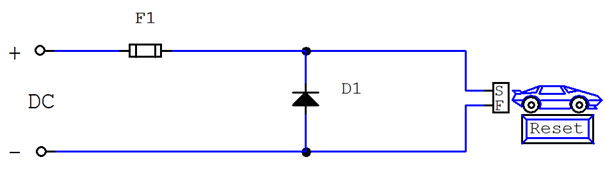
\includegraphics[width=0.7\textwidth]{diode/figurer/DiodeLading.png}
		\caption{Enkel ladekrets med sikring}
		\label{fig:diodeLading}
	\end{figure}
	
\end{question}

\vspace{0.5cm} % Add space after the solution

\begin{solution}[name=Løsningsforslag oppgave]
	
Under vanlige driftsforhold og korrekt polaritet så vil dioden stå i sperreretning og det vil ikke bevege seg strøm gjennom den. Dersom man kobler feil polaritet som beskrevet i oppgaven så vil dioden befinne seg i lederetning. Siden dioden har en relativt lav motstand i lederetning, og strømmen naturlig velger veien tilbake til den negativ polaritet med minst motstand, som vil strømmen bevege seg gjennom dioden. Strømmen vil være opp mot maksimal kortslutningsstrøm for kilden og $>>$\footnote{Tegnet betyr mye større enn. Eksempel: $9\cdot10^{9}>>1\cdot10^{-10}$} enn nominell strøm. Det igjen vil føre til at sikringen løser. Et eksempel er vist i \ref{fig:diodeLadingSol}.
	\begin{figure}[H]
	\centering
	\includegraphics[width=0.7\textwidth]{diode/figurer/DiodeLading–SOL.png}
	\caption{Løsning på enkel ladekrets med sikring}
	\label{fig:diodeLadingSol}
\end{figure}

	
\end{solution}




\begin{question}[name=Oppgave, topic=dioder]
	Din elektriske sportsbil får tilført en likespenning fra en nå oppgradert hurtiglader sammenlignet med løsningen vist i Figur \ref{fig:diodeLadingG}. Hva skjer nå dersom spenningskilden blir koblet med feil polaritet?
	
	\begin{figure}[H]
		\centering
		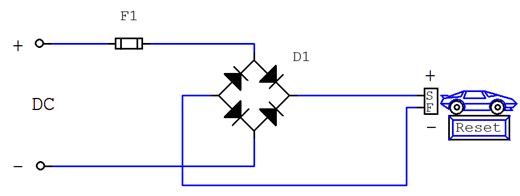
\includegraphics[width=0.7\textwidth]{diode/figurer/GretzLading.png}
		\caption{Ladekrets med brolikeretter}
		\label{fig:diodeLadingG}
	\end{figure}
	
\end{question}

\vspace{0.5cm} % Add space after the solution

\begin{solution}[name=Løsningsforslag oppgave]
Det skjer ingenting siden bro-likeretteren snur polariteten og sørger for riktig polaritet til bilen. I Figur \ref{fig:BroLadingSol} kan man observere retningen på strømmen under nominelle forhold, og i Figur \ref{fig:BroLadingSol2} kan man observere hva som skjer dersom man bytter polaritet.

\begin{figure}[H]
	\centering
	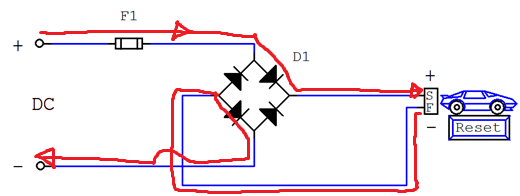
\includegraphics[width=0.7\textwidth]{diode/figurer/GretzLadingVanlig-SOL.png}
	\caption{Løsning på ladekrets under nominelle forhold}
	\label{fig:BroLadingSol}
\end{figure}
	
\begin{figure}[H]
	\centering
	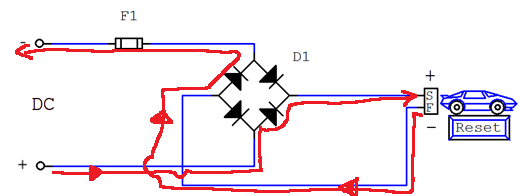
\includegraphics[width=0.7\textwidth]{diode/figurer/GretzLadingFeil-SOL.png}
	\caption{Løsning på ladekrets med feil polaritet}
	\label{fig:BroLadingSol2}
\end{figure}	
	
	
\end{solution}





\vspace{0.5cm} % Add space after the solution

%DUPLIKAT
\begin{comment}
	innhold...

\begin{question}[name=Oppgave, topic=dioder]
	Hvilken av kretsene vist i \ref{fig:3kretser} er koblet slik at dioden står i lederetning?
	
	\begin{figure}[H]
		\centering
		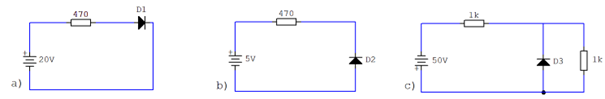
\includegraphics[width=0.9\textwidth]{diode/figurer/3Kretser.png}
		\caption{Tre forskjellige diodekretser}
		\label{fig:3kretser}
	\end{figure}
	
\end{question}

\vspace{0.5cm} % Add space after the solution

\begin{solution}[name=Løsningsforslag oppgave]
	Krets a) og c)
\end{solution}
\vspace{0.5cm} % Add space after the solution

\end{comment}


\begin{question}[name=Oppgave, topic=dioder]
Beregn strømmen i kretsen som er vist i Figur \ref{fig:2kilder}.
	\begin{figure}[H]
			\centering
			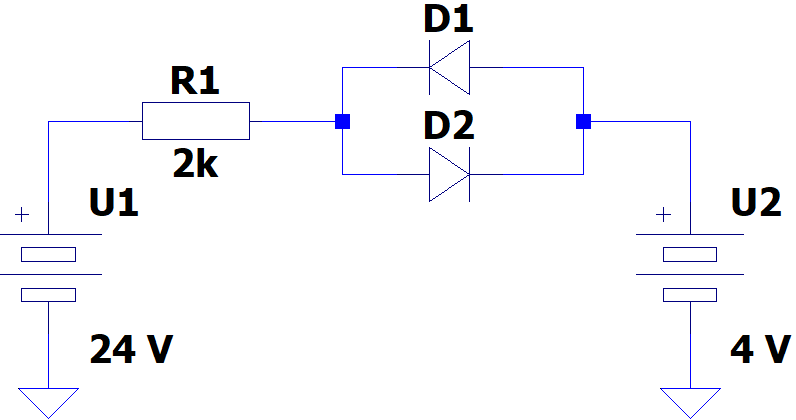
\includegraphics[width=0.7\textwidth]{diode/figurer/kretsM2kilder.png}
			\caption{Diodekrets med to kilder}
			\label{fig:2kilder}
		\end{figure}

\end{question}

\vspace{0.5cm} % Add space after the solution

\begin{solution}[name=Løsningsforslag oppgave]
Diode $D1$ er koblet i sperreretning og kan betraktes som brudd. Strømmen gjennom $R_1$ beregnes ut fra kretsens spenningsfall.

\[I_{tot}=\frac{U_1-U_2-U_{diode}}{R_1}=\frac{24-4-0,7}{2\cdot10^3}=9,65 [mA]\]
	
\end{solution}
\vspace{0.5cm} % Add space after the solution


\begin{question}[name=Oppgave, topic=dioder]
Gitt det påtrykte signalet vist i Figur \ref{fig:20Sine}, beregn den maksimale strømmen og spenning for kretsen vist i Figur \ref{fig:acKrets}.
\begin{figure}[H]
	
	\begin{minipage}[c]{0.45\linewidth}
		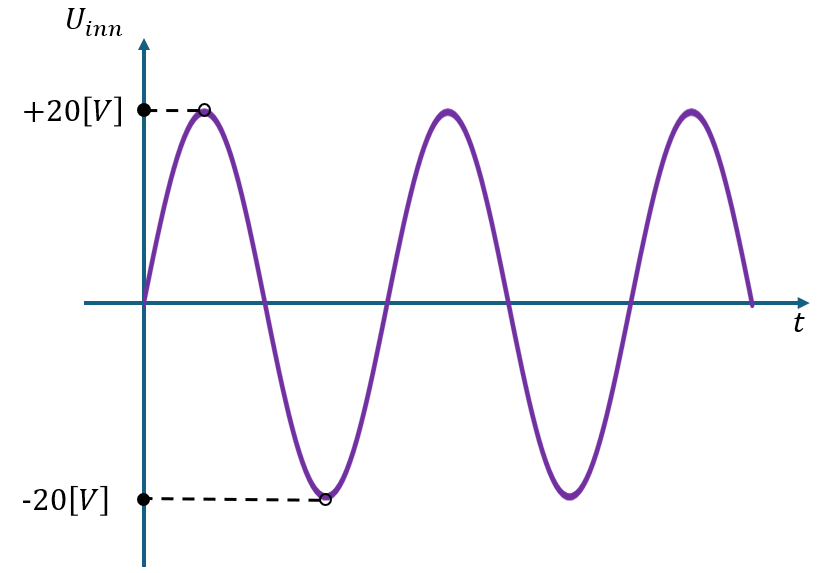
\includegraphics[width=\linewidth]{diode/plot/20Sinus.png}
		\caption{Signal på inngangen}
		\label{fig:20Sine}
	\end{minipage}
	\hfill
	\begin{minipage}[c]{0.45\linewidth}
		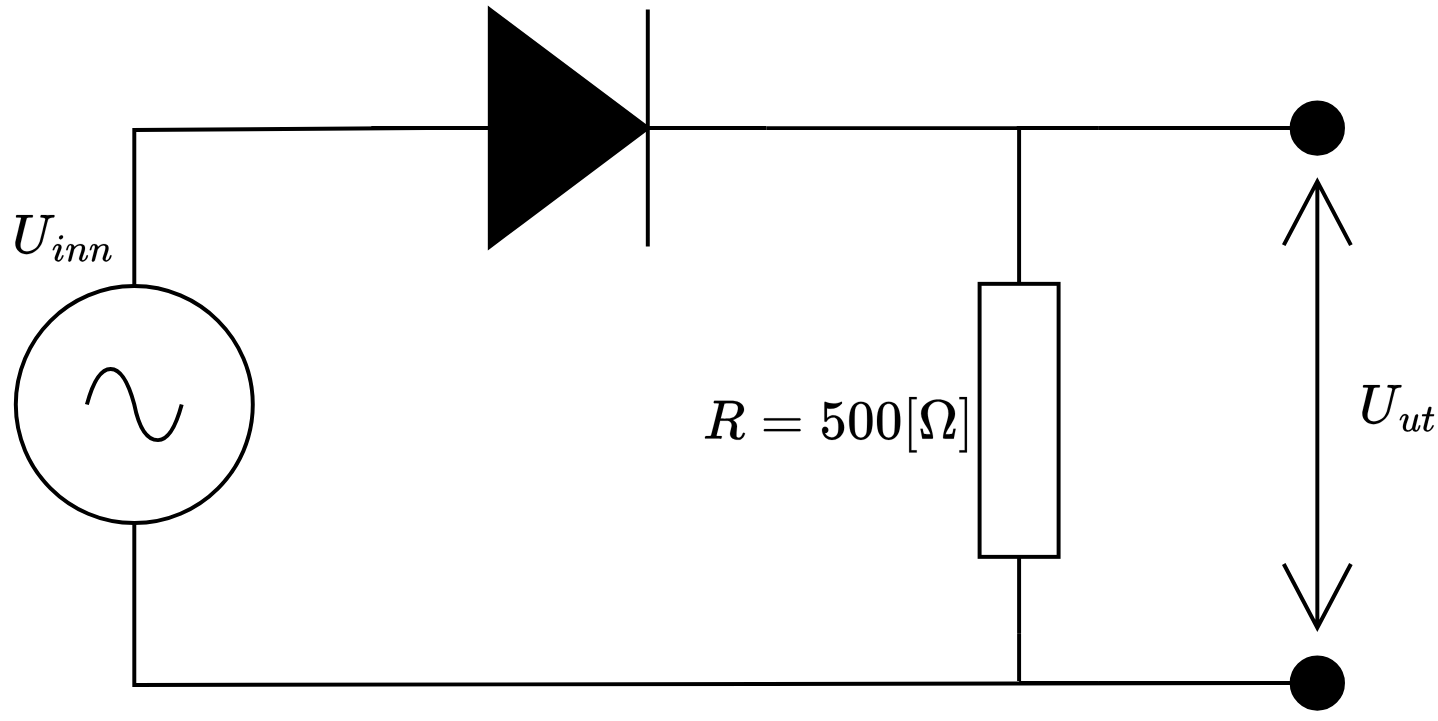
\includegraphics[width=\linewidth]{diode/figurer/diodeSinus.png}
		\caption{Enkel diodekrets}
		\label{fig:acKrets}
	\end{minipage}
\end{figure}
	
\end{question}

\vspace{0.5cm} % Add space after the solution

\begin{solution}[name=Løsningsforslag oppgave]
Beregner maksimale spenningen $U_{ut_{peak}}$
\[U_{ut_{peak}}=U_{inn_{peak}}-U_{diode_{peak}}=20-0,7=19,3 [V]\]

Finner så den høyeste strømmen i kretsen  $I_{peak}$
\[I_{peak}=\frac{U_{ut_{peak}}}{R}=\frac{19,3}{500}=38,6 [mA]\]

\end{solution}
\vspace{0.5cm} % Add space after the solution






\begin{question}[name=Oppgave, topic=dioder]
Tegn hvordan spenningen over dioded i Figur \ref{fig:enklAcDiode} endrer seg med tiden for to hele perioder.
	\begin{figure}[H]
	\centering
	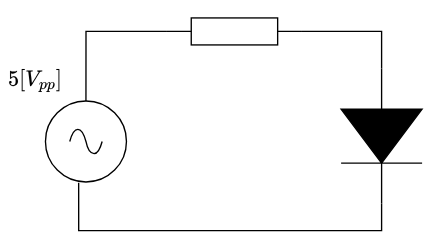
\includegraphics[width=0.5\textwidth]{diode/figurer/ACdiode.png}
	\caption{Enkel diodekrets}
	\label{fig:enklAcDiode}
\end{figure}
	
\end{question}

\vspace{0.5cm} % Add space after the solution

\begin{solution}[name=Løsningsforslag oppgave]
	\begin{figure}[H]
	\centering
	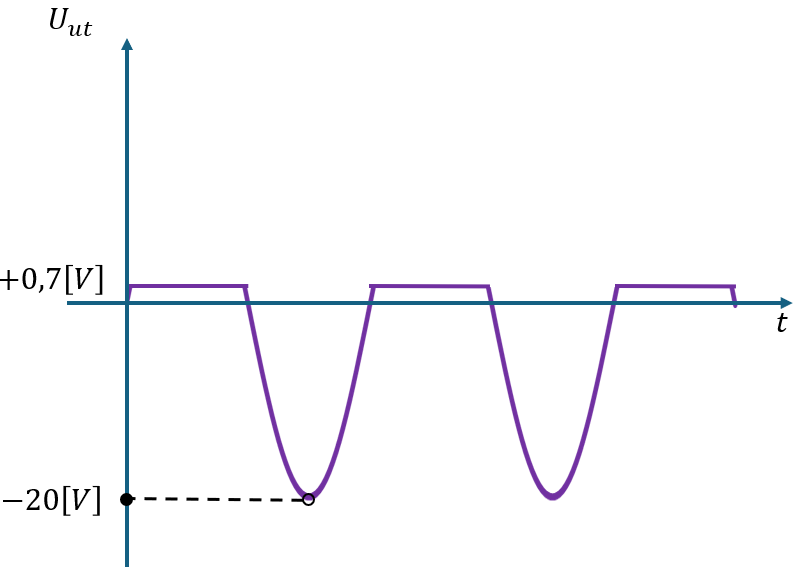
\includegraphics[width=0.5\textwidth]{diode/figurer/ACdiode-LOS.png}
	\caption{Løsning på enkel diodekrets}
	\label{fig:enklAcDiodeLOS}
\end{figure}
	
\end{solution}
\vspace{0.5cm} % Add space after the solution